\section{Stati elettronici}
\subsection{cenni teorici}

Ci interesseremo ora delle transizioni elettroniche, focalizzando la nostra attenzione
su un gruppo cromoforo di particolare importanza in chimica organica, il carbonile.

Come \'e noto, il momento angolare totale di spin di una molecola \'e
rappresentato dal numero quantico S. Tale grandezza vettoriale pu\`o essere 
calcolata come somma dei singoli contributi di spin elettronici: se in un 
semplicistico caso bielettronico, le due particelle possedessero spin opposti,
il momento di spin totale sarebbe $ \half - \half = 0 $. Se invece le due 
particelle possedessero spin parallelo, il numero quantico totale S sarebbe 
$ \half + \half = 1 $. Dal momento che la molteplicit\`a dello stato \'e 
valutabile in $ 2 S + 1 $, ne consegue che per il primo caso si avr\`a uno
stato di \textbf{singoletto}, mentre nel secondo uno stato di \textbf{tripletto}.

La maggior parte delle molecole organiche ha uno stato base di
closed shell, quindi uno stato di singoletto ($S_{0}$). Eccitazioni elettroniche
della molecola possono condurre sia a stati di tripletto $T_{1}$ sia a stati di
singoletto $S_{1}$, a seconda che l'eccitazione produca o meno l'inversione
dello spin.

Le transizioni $ S \rightarrow T $ sono virtualmente proibite, dal
momento che nell'integrale di transizione per la sola parte elettronica

\beqas
\int{\psi_{el'}\overrightarrow{d_{e}}\psi_{el}} & = &
\int{\varphi_{el'}\overrightarrow{d_{e}}\varphi_{el}}
\int{\mathcal{S}_{el'} \mathcal{S}_{el}}
\eeqas

vede la funzione di spin integrare a parte, dato che il momento
dipolare elettronico $\overrightarrow{d_{e}}$ \'e un operatore 
puramente spaziale. 
Come conseguenza, siccome le funzioni di singoletto e di tripletto
sono ortogonali, l'integrale condotto sullo spin \'e nullo e la
transizione di \textit{Inter System Crossing} \'e spin proibita.

Transizioni che avvengono tra stati della medesima molteplicit\`a di spin
sono invece consentite (a meno di una proibizione sulla simmetria nella
parte spaziale dell'integrale) e vengono denominate \textit{Internal
Conversion}.

\subsection{Un esempio pratico: la formaldeide}

Come esempio del cromoforo carbonile, utilizzeremo la formaldeide. Il
suo schema orbitalico vede un carbonio ibrido $sp^2$ che lega col
rimanente orbitale $2p_x$ per via $\pi$ con l'orbitale di adatta
simmetria dell'ossigeno. Un orbitale p dell'ossigeno resta come orbitale
di non legame.
\begin{center}
\vspace{0.3cm}
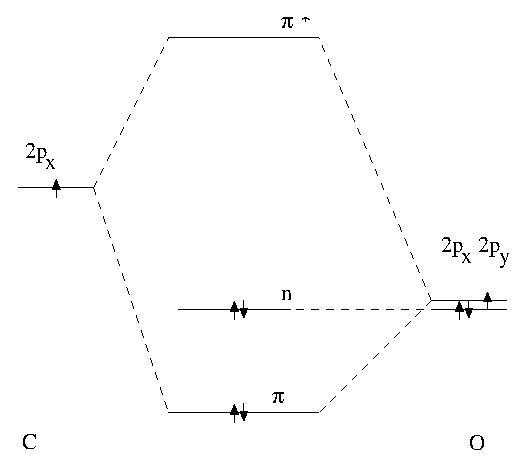
\includegraphics{../immagini/formaldeide.eps} 
\vspace{0.3cm}
\end{center}

L'occupazione elettronica vede doppiamente occupato l'orbitale di legame
$\pi$ e l'orbitale di non legame $n$, che resta sull'ossigeno come doppietto 
non legato.

Tale schema rende possibili due tipi di transizione: una transizione
dall'orbitale legante all'orbitale antilegante ($ \pi \rightarrow
\pistar $) e una transizione dall'orbitale di non legame all'orbitale di
antilegame ($ n \rightarrow \pistar $). Dal momento che nel ground state
tutti gli elettroni sono appaiati, ne deriva che tale stato \'e di
singoletto. L'eccitazione elettronica pu\`o condurre a due differenti
stati, ciascuno con diversa molteplicit\`a di spin.

Una transizione che preservi il momento angolare totale, conduce ad uno
stato di singoletto. In tale caso, l'integrale di sovrapposizione tra le
due funzioni di spin vale
\beqas
% first eq
\integral{\mathcal{S}_0}{\mathcal{S}_1} & = & 
\half \left[
\integral{\alpha(1)\beta(2)-\alpha(2)\beta(1)}{\alpha(1)\beta(2)-\alpha(2)\beta(1)}
\right] \\
% second eq
& = & \half \left[ \integral{\alpha(1)}{\alpha(1)} \integral{\beta(2)}{\beta(2)} \right. \\
& & - 2 \integral{\alpha(1)}{\beta(1)} \integral{\alpha(2)}{\beta(2)} \\
& & + \left. \integral{\alpha(2)}{\alpha(2)} \integral{\beta(1)}{\beta(1)} \right] \\
% third eq
& = & 1
\eeqas
dal momento che $ \integral{\alpha}{\alpha} = \integral{\beta}{\beta}
= 1 $ per ortonormalit\`a.

Al contrario, una transizione da uno stato di singoletto ad uno stato di
tripletto non \'e spin consentita
\beqas
% first eq
\integral{\mathcal{S}_0}{\mathcal{T}_1} & = & 
\frac{1}{\sqrt{2}} \left[
\integral{\alpha(1)\beta(2)-\alpha(2)\beta(1)}{\alpha(1)\alpha(2)} \right] \\
%second eq
& = & \frac{1}{\sqrt{2}} \left[ \integral{\alpha(1)}{\alpha(1)}
\integral{\beta(2)}{\alpha(2)} - \integral{\alpha(2)}{\alpha(2)}
\integral{\beta(1)}{\alpha(1)} \right] \\
& = & 0
\eeqas
sempre per ortonormalit\`a delle funzioni di spin ( $
\integral{\alpha}{\beta} = \integral{\beta}{\alpha} = 0 $ ).

Questo tipo di approccio dovrebbe portare a concludere che l'intensit\`a della
transizione \'e nulla. In realt\`a, tale trattazione \'e alquanto semplicistica. 
Nell'eventualit\`a che le funzioni di spin siano puramente di singoletto o 
puramente di tripletto, allora tale trattazione conduce al risultato
teorico ipotizzato, ma solitamente la purezza di spin non \'e totale, e 
funzioni di singoletto possono avere certo carattere di tripletto e 
viceversa. Questo grazie all'accoppiamento tra il momento angolare di 
spin e il momento angolare orbitale.

Dal momento che tale effetto \'e blando, possiamo trattarlo
perturbativamente: l'hamiltoniano del nostro sistema sar\`a quindi
trattato come 
$$
\ham = \ham^0 + \ham'
$$
dove $\ham'$ \'e responsabile dell'accoppiamento tra il momento angolare
di spin e il momento angolare orbitale. Per la teoria perturbativa, la
nostra funzione spin-elettronica pu\`o essere espressa come 
$$
\psin = \psin^0 + \sumidxprm{k} a_k \psik^0 
$$
dove i coefficienti $a_k$ sono ricavati perturbativamente dalla
relazione
$$
a_k = \frac{\braket{\psik^0}{\ham'}{\psin^0}}{E_n^0-E_k^0}
$$
Integrando sul momento dipolare di transizione, otterremo
$$
\mu_{nm} = \mu_{nm}^0 + \sumidxprm{k}a_k\mu_{km}^0
$$
La transizione tra stati puri $\mu_{nm}^0$ quindi pu\`o essere nulla, ma
il momento di transizione totale $\mu_{nm}$ pu\`o essere diverso da zero
in virt\`u della presenza del termine perturbativo, che contribuisce a
mescolare gli stati di tripletto e singoletto. L'intensit\`a di tale
mescolamento \'e tanto maggiore quanto maggiore \'e la costante di
accoppiamento spin-orbita, che in spettroscopia atomica dipende
strettamente dal numero atomico. Nel caso molecolare, tale dipendenza \'e
approssimativamente ancora valida, e quindi molecole organiche che presentano 
tra gli elementi costitutivi atomi pesanti saranno maggiormente soggette a
consentire transizioni spin proibite, che diventano in questo modo pi\`u
intense, ma in ogni caso considerevolmente pi\`u deboli (di qualche
ordine di grandezza) delle spin ammesse.

Una volta che una molecola viene eccitata ad uno stato elettronico a maggiore
energia, lo stato instabile che se ne ottiene tende ad evolvere
secondo vari processi, al fine di sgravare l'energia eccedente e tornare
allo stato base. Dal punto di vista fotochimico, sono di notevole
interesse i processi radiativi \textbf{fluorescenza} e
\textbf{fosforescenza}.

La fluorescenza coinvolge stati eccitati della medesima molteplicit\`a
dello stato base. In tale caso, il rilassamento avviene su scale
temporali ridotte e con intensit\`a elevata.
Nel caso della fosforescenza, invece, il rilassamento prevede una
transizione tra stati di differente molteplicit\`a (nei casi pi\`u
frequenti, da uno stato di tripletto eccitato, popolato via Inter System
Crossing grazie all'accoppiamento spin-orbita, al ground state di
singoletto). In virt\`u di ci\`o, il rilassamento avviene su scale
temporali decisamente pi\`u lunghe (anche nell'ordine dei secondi).

\subsection{Regole di selezione per l'Inter System Crossing}

Abbiamo potuto accertare che, attraverso una parte perturbativa, la
transizione tra stati di differente molteplicit\`a \'e consentita.
Dal momento che questo contributo ha le stesse propriet\`a di simmetria
delle rotazioni $R_x, R_y, R_z$, al fine di determinare se una
transizione ISC \'e possibile, basta valutare gli integrali
$$
\braket{\psin}{\ham{'}_{x}}{\psim}, \braket{\psin}{\ham{'}_{y}}{\psim}, \braket{\psin}{\ham{'}_{z}}{\psim}
$$
Come regola generale per le transizioni che interessano il gruppo
carbonilico, \'e possibile dimostrare che i rilassamenti ISC $ ^1(n \rightarrow
\pistar) \rightarrow \: ^3 (\pi \rightarrow \pistar) $ e $ ^1(\pi
\rightarrow \pistar) \rightarrow \:^3(n \rightarrow \pistar) $ sono
consentiti. Tutti gli altri riarrangiamenti sono proibiti.

\section{Teoria MCSCF}

\subsection{Introduzione}

Il successo della teoria HF \'e dovuto alla sua relativa efficienza
applicato a sistemi closed shell. Grazie a tale teoria, \'e possibile
ottenere un set spinorbitalico ottimale (orbitali canonici) da
utilizzare in successive trattazioni.
Si pu\`o ricavare che, al fine di minimizzare l'energia di un 
monodeterminte $\Phi = \detsl{\psi_1 \ldots \psi_n} $, deve essere
$$
\braket{\Phi}{\ham}{\Phi_i^a} = 0 \mbox{ (teorema di Brillouin)}
$$
ovvero non ci deve essere interazione tra lo stato $\Phi$ e una sua
singola eccitazione. Questo conduce, grazie alle regole di Slater,
alla definizione dell'operatore di Hartree-Fock $\hat{F}$ e alla 
relazione tra spinorbitali
$$
\braket{\psia}{\hat{F}}{\psii} = 0
$$

Questo implica che $\hat{F}\psii$ \'e uno spinorbitale totalmente
ortogonale allo spazio degli spinorbitali virtuali, e come tale
appartiene allo spazio degli occupati. Da ci\`o si ottiene
$$
\hat{F}\psii = \sumonen{j}\psij\epsilon_{ji}
$$

Esister\`a quindi un particolare set spinorbitalico che, oltre a
soddisfare il teorema di Brillouin (e quindi rendere minima l'energia
HF), diagonalizza anche la matrice $\epsilon_{ji}$. Questi spinorbitali
sono detti \textbf{canonici}. 

I valori diagonali di tale matrice prendono il nome di \textbf{energie
orbitaliche}, e per il teorema di Koopmans
$$
E_+^i-E_0 = -\epsilon_i
$$
rappresentano approssimativamente l'energia di ionizzazione in gioco
durante la rimozione di un elettrone dall'orbitale \textit{i}-esimo.

Tale trattazione \'e tuttavia insoddisfacente durante l'analisi di
legami in via di dissociazione. La principale approssimazione deriva dal
supporre che la configurazione della molecola in studio sia data
esclusivamente dal monodeterminante di Slater considerato. 

Per questa ragione, occorre descrivere la molecola come una \textbf{Multi
Configurazione} di determinanti. Durante la rottura di legami, ma anche
in molti altri casi, specie quando stati quasi degeneri entrano in
gioco, una descrizione monodeterminantale non \'e sufficiente a garantire
che l'energia HF sia una sufficiente approssimazione dell'energia vera
dello stato.

\subsection{Un caso semplice: l'idrogeno}

La molecola di idrogeno \'e il caso accademico pi\`u noto. Gli orbitali
molecolari sono comunemente scritti come LCAO dei due atomi, per cui:
$$
\varphi_1=N \left(1s_a + 1s_b \right)
$$

dal momento che tale orbitale spaziale \'e doppiamente occupato,
l'orbitale molecolare sar\`a ovviamente
$$
\Phi_1 = \varphi_1(1) \varphi_1(2) \frac{\alpha \beta - \beta \alpha}{\sqrt{2}}
$$
Utilizzando tale descrizione elettronica per l'equilibrio, i risultati
ottenuti sono in buon accordo con il dato sperimentale, tuttavia la
funzione resta la stessa a qualsiasi distanza i due atomi si trovino.
Svolgendo il prodotto della funzione $ \Phi_1 $ \'e possibile riconoscere
una componente covalente (che vede gli elettroni equamente distribuiti
su entrambi gli atomi) e una componente ionica (che vede la coppia
elettronica in possesso di un solo atomo). Tale trattazione assegna alle
componenti lo stesso peso, a qualsiasi distanza interatomica.
Come conseguenza, l'energia SCF ottenuta da tale trattazione \'e
totalmente errata, e l'errore aumenta al crescere della distanza
interatomica
\begin{center}
\vspace{0.3cm}
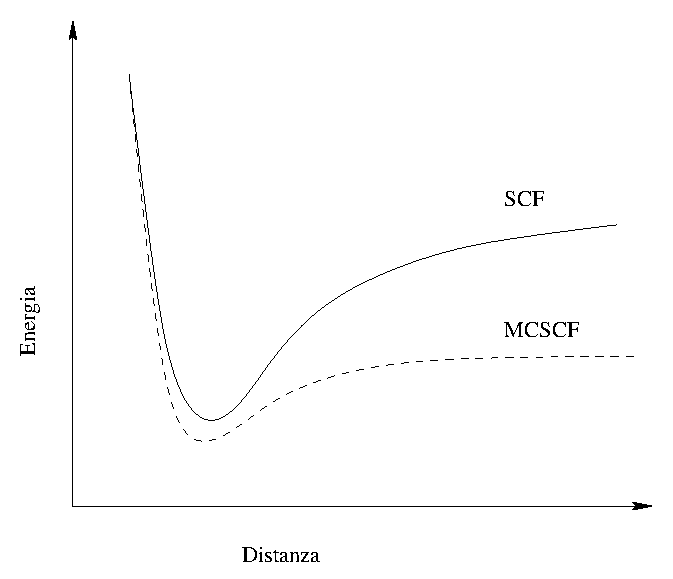
\includegraphics{../immagini/SCF-MCSCF.eps} 
\vspace{0.3cm}
\end{center}

Possiamo migliorare la trattazione ipotizzando la funzione descrittiva
come una combinazione lineare di stati, aggiungendo l'antilegame
$$
\varphi_2=N_2 \left( 1s_a - 1s_b \right)
$$

e scrivendo quindi la funzione d'onda MC
$$
\Psi_{MC} = c_1 \Phi_1 + c_2 \Phi_2
$$
Questa funzione presenta sia carattere di legame sia carattere di
antilegame, e mostra il corretto comportamento asintotico.

In questo semplice caso, abbiamo due elettroni che vengono distribuiti
su 2 orbitali. Purtroppo anche in molecole semplici, come ossigeno e
azoto, il numero di orbitali e di elettroni con cui trattare \'e abbastanza 
elevato. Questo comporta che una trattazione completa delle possibili 
distribuzioni elettroniche richiede tempi di calcolo notevoli. Al fine 
di semplificare, si \'e introdotto un metodo alternativo, che prevede la 
suddivisione dello spazio orbitalico in 3 insiemi: 
\begin{itemize}
\item orbitali virtuali, sempre vuoti
\item orbitali attivi, parzialmente riempiti
\item orbitali inattivi, completamente riempiti.
\end{itemize}

Il metodo si basa sulla semplificazione di considerare le possibili
disposizioni degli elettroni solo internamente allo spazio degli
orbitali attivi. Questo riduce la complessit\`a computazionale, ma
introduce la necessit\`a di scegliere in modo ottimale il set degli 
orbitali attivi.

\subsection{Metodo MCSCF e seconda quantizzazione}

Al fine di utilizzare i metodi numerici MCSCF, sar\`a utile approfondire
i metodi in seconda quantizzazione.

Si abbia un set spinorbitalico $ \left\{ \psi_1 \psi_2
\ldots \psi_{2n} \right\} $ dato da $n$ orbitali spaziali. Usando
tali spinorbitali, \'e possibile costruire un generico determinante di
Slater, definendo solo il numero di occupazione di ogni spinorbitale
$$
\Phi = \ket{1,1,0,0,1}
$$
che secondo un formalismo analogo \'e scrivibile come
$$
\Phi = \detsl{\psi_1 \psi_2 \psi_5}
$$
Attraverso gli operatori di creazione e distruzione \'e possibile
aggiungere o rimovere uno spinorbitale ad un determinante, secondo le
seguenti regole (analizzate con il doppio formalismo). Per il distruttore, 
se lo spinorbitale bersaglio \'e presente
\beqas
\destr{i} \ket{m_1,m_2,\ldots,m_{i-1},1,m_{i+1},\ldots,m_{2n}} & = &
(-1)^{\sum_{j=1}^{i-1}m_j} \ket{m_1,m_2,\ldots,m_{i-1},0,m_{i+1},\ldots,m_{2n}} \\
\destr{i}
\detsl{\psi_1,\psi_2,\ldots,\psi_{i-1},\psi_i,\psi_{i+1},\ldots,\psi_{2n}} & = &
(-1)^{p_i} \detsl{\psi_1,\psi_2,\ldots,\psi_{i-1},\psi_{i+1},\ldots,\psi_{2n}}
\eeqas
dove $p_i$ \'e il numero di trasposizioni necessarie a portare l'orbitale
bersaglio in prima posizione nel determinante.
Nel caso lo spinorbitale sia assente, il risultato \'e zero.

Per il costruttore, se lo spinorbitale bersaglio \'e assente
\beqas
\constr{i} \ket{m_1,m_2 \ldots m_{i-1},0,m_{i+1} \ldots m_{2n}} & = &
(-1)^{\sum_{j=1}^{i-1}m_j} \ket{m_1,m_2 \ldots m_{i-1},1,m_{i+1} \ldots m_{2n}} \\
\destr{i} \detsl{\psi_1,\psi_2,\ldots,\psi_{i-1},\psi_{i+1},\ldots,\psi_{2n}} & = &
(-1)^{p_i}
\detsl{\psi_1,\psi_2,\ldots,\psi_{i-1},\psi_{i},\psi_{i+1},\ldots,\psi_{2n}}
\eeqas
in caso contrario (spinorbitale gi\`a presente), il risultato \'e zero.

\'E utile ricordare le regole di anticommutazione per gli operatori di
creazione e distruzione
\beqas
\constr{i}\constr{j}+\constr{j}\constr{i} = 0 \\
\destr{i}\destr{j}+\destr{j}\destr{i} = 0 \\
\constr{i}\destr{j}+\destr{j}\constr{i} = \delta_{ij}
\eeqas
come anche l'operatore di eccitazione/diseccitazione $\constr{i}\destr{j}$ che porta un
elettrone dall'orbitale j all'orbitale i
$$
\constr{i}\destr{j} \ket{m_1,m_2,\ldots,0_i,\ldots,1_j,\ldots} =
(-1)^{\sum_{k=i+1}^{j-1}m_k} \ket{m_1,m_2,\ldots,1_i,\ldots,0_j,\ldots}
$$
Possiamo anche definire un operatore spin traced
$$
E_{ij} = \left( \constr{i\alpha}\destr{j\alpha} +
\constr{i\beta}\destr{j\beta} \right)
$$
Questo operatore si riferisce agli n orbitali molecolari spaziali,
indipendentemente dal fattore di spin.
Valgono le propriet\`a
\begin{itemize}
\item $ \left[ E_{ij}, E_{kl} \right] = E_{il}\delta_{jk} -
E_{kj}\delta_{il} $
\item $ E^{+}_{ij} = E_{ji} $
\end{itemize}

\subsection{Operatori in seconda quantizzazione}

Mediante il formalismo della seconda quantizzazione, \'e possibile
scrivere gli operatori quantistici secondo un differente approccio.
Un generico operatore monoelettronico pu\`o essere espanso sulla base di
operatori di creazione e distruzione
$$
\hat{F} = \sumidx{i,j} F_{ij} \constr{i}\destr{j}
$$
dove $F_{ij}$ \'e l'elemento di matrice
$$
F_{ij} = \int \! \psii^{*}(x)\hat{F}(x)\psij(x) \: dx
$$

Sommando in modo opportuno (abbinandoli) i vari termini della
sommatoria, si pu\`o ottenere
$$
\hat{F} = \sumidx{i,j} F_{ij}E_{ij}
$$
dove gli indici $i$ e $j$ ora sono indici di orbitale puramente spaziale
e l'integrale $F_{ij}$ \'e ora definito su una base spaziale.

Analogamente possiamo definire un operatore bielettronico
$$
\hat{G} = \sumidx{i,j,k,l} g_{ijkl} \constr{i}\constr{j}\destr{l}\destr{k}
$$
dove $g_{ijkl}$ \'e l'integrale
$$
g_{ijkl} = \int \! \! \! \! \int \! \psii^*(x_1) \psij^*(x_2) \hat{G}(x_1,x_2) \psik
\psil \, dx_1 dx_2
$$

Sommando sullo spin, dopo alcune manipolazioni, \'e possibile ottenere il
risultato
$$
\hat{G} = \half \sumidx{i,j,k,l} g_{ijkl} \left( E_{ij} E_{kl} -
\delta_{jk} E_{il} \right)
$$
dove, al solito, gli indici corrono ora su orbitali puramente spaziali.

In conclusione, l'hamiltoniano in seconda quantizzazione \'e scrivibile
come
$$
\ham = \sumidx{i,j} h_{ij} E_{ij} + \half \sumidx{i,j,k,l} g_{ijkl}
\left( E_{ij} E_{kl} - \delta_{kj} E_{il} \right)
$$

\subsection{Trasformazione di base}

Al fine di rendere minima l'energia, occorre effettuare una trasformazione 
sia sui coefficienti della nostra funzione MC, sia sulla base spinorbitalica 
su cui costruiamo i vari determinanti.

Tali trasformazioni possono essere viste come rotazioni in uno spazio
ortonormale, attuate da un operatore opportuno. Dal momento che la
rotazione non cambia la dimensionalit\`a della base, il risultato
appartiene ancora allo spazio delle funzioni spinorbitaliche di
partenza, e come tale \'e esprimibile come una opportuna combinazione
lineare dei vettori della base iniziale
$$
\mathbf{\varphi}' = \mathbf{\varphi}\mathbf{U}
$$
dove $\mathbf{\varphi}$ \'e un vettore riga contenente gli spinorbitali di
partenza, $\mathbf{\varphi}'$ \'e la base ottenuta dalla trasformazione e
$\mathbf{U}$ \'e una matrice unitaria che attua la trasformazione stessa.

Dal momento che viene attuata una trasformazione sulla base, \'e
indiscutibile che anche gli operatori di creazione e distruzione
andranno incontro ad una trasformazione. \'E possibile esprimere la
trasformazione nello stesso modo, oppure attraverso la relazione
$$
\constr{i}{}^\prime = e^{\left(-\hat{T}\right)} \constr{i}
e^{\left(\hat{T}\right)}
$$
e analogamente per il distruttore. L'operatore $\hat{T}$ \'e un operatore
antihermitiano, che pu\`o essere espanso, come un operatore
monoelettronico, nella forma
$$
\hat{T}=\sumidx{ij}T_{ij}\constr{i}\destr{j}
$$
creazione e distruzione, per ottenere una matrice $\mathbf{T}$
antihermitiana (ovvero vale $\mathbf{T}^{+} = - \mathbf{T}$)

\pagebreak
Si dimostra che \'e possibile trasformare un generico determinante di 
Slater applicando l'operatore $e^{-\hat{T}}$:
\beqas
% 
\ket{m'}= a{'}_i^+ a{'}_j^+ \ldots\vacuum & = &
e^{\left(-\hat{T}\right)} \constr{i} e^{\left(\hat{T}\right)}
e^{\left(-\hat{T}\right)}\constr{j} e^{\left(\hat{T}\right)}\ldots\vacuum
\\
% 
& = & e^{\left(-\hat{T}\right)}\constr{i} \constr{j}\ldots\vacuum \\
%
& = & e^{\left(-\hat{T}\right)}\ket{m}
\eeqas

Dal momento che la trasformazione attuata sugli orbitali
avviene esclusivamente sulla parte spaziale, la matrice di
trasformazione $\mathbf{T}$ \'e partizionata in 4 sottomatrici
$$
\mathbf{T} = \left(
\begin{array}{cc}
\mathbf{T}_{\alpha\alpha} & \mathbf{T}_{\alpha\beta} \\
\mathbf{T}_{\beta\alpha} & \mathbf{T}_{\beta\beta}
\end{array}
\right)
$$

Se non si effettua mescolamento tra orbitali con occupazione $\alpha$ e
orbitali con occupazione $\beta$, i termini delle sottomatrici fuori 
diagonale $\mathbf{T}_{\alpha\beta}$ e $\mathbf{T}_{\beta\alpha}$ sono 
nulli, e dal momento che le trasformazioni sono le stesse 
per lo stesso set spaziale, $\mathbf{T}_{\alpha\alpha} = \mathbf{T}_{\beta\beta}$.
Con queste relazioni, l'operatore $\hat{T}$ risulta
\beqas
%
\hat{T} & = & \sumidx{i,j} \left( T_{ij}^{\alpha\alpha} \constr{i\alpha}
\destr{j\alpha} 
+ T_{ij}^{\alpha\beta} \constr{i\alpha} \destr{j\beta}
+ T_{ij}^{\beta\alpha} \constr{i\beta} \destr{j\alpha}
+ T_{ij}^{\beta\beta} \constr{i\beta} \destr{j\beta} \right) \\
%
& = & \sumidx{i,j} T_{ij} \left( \constr{i\alpha} \destr{j\alpha} +
\constr{i\beta} \destr{j\beta} \right) \\
%
& = & \sumidx{i,j} T_{ij}E_{ij}
\eeqas
e dal momento che T \'e una matrice antihermitiana, $T_{ij} = -T_{ji}$ e
quindi
$$
\hat{T} = \sumidx{i>j} T_{ij}\left(E_{ij} - E_{ji}\right) 
= \sumidx{i>j} T_{ij} E_{ij}^-
$$

\subsection{Le equazioni del metodo MCSCF. Metodo Newton-Raphson}

L'ottimizzazione di una funzione d'onda multiconfigurazionale, prevede
di modificare sia gli orbitali base, sia i coefficienti della combinazione
lineare di determinanti.

L'assunto di partenza \'e considerare l'energia del sistema $E$ come
funzione di un vettore di parametri $\mathbf{p}$, e quindi espandere
tale dipendenza in serie di Taylor attorno un punto $\mathbf{p}_0$ posto
uguale a $0$. Si avr\`a
$$
E(\mathbf{p}) = E(0) + \sumidx{i} \left( \frac{\partial E}{\partial
p_i}\right)_0 p_i + \half \sumidx{i,j} p_i \left( \frac{\partial^2 E}{\partial
p_i \partial p_j} \right)_0 p_j + \ldots
$$
che in notazione matriciale diventa
$$
E(\mathbf{p}) = E(0) + \mathbf{g}^+\mathbf{p} + \half
\mathbf{p}^+\mathbf{H}\mathbf{p} + \ldots
$$
dove $\mathbf{g}$ \'e un vettore detto \textit{gradiente energia} e
$\mathbf{H}$ \'e la \textit{matrice Hessiana} dell'energia.

Affinch\`e si abbia un minimo, la derivata prima dell'energia rispetto 
a tutti i parametri deve essere zero, ovvero il vettore gradiente nullo.
Per risolvere tale problema, si ricorre ad una procedura iterativa 
che prevede di risolvere l'equazione lineare
$$
\mathbf{g} + \mathbf{Hp} = \mathbf{0} 
$$

\subsection{Ottimizzazione dei parametri e degli orbitali}

L'ottimizzazione dei parametri e degli orbitali passa attraverso l'uso
di operatori unitari. Abbiamo gi\`a avuto modo di incontrare l'operatore
$\hat{T}$, che attua una rotazione dello spazio orbitalico. Analogamente,
\`e possibile definire un operatore unitario $\hat{S}$ che attua una
trasformazione sui coefficienti della combinazione lineare.

L'energia dello stato MC $\ket{0}$ sar\`a quindi definita
$$
E(\mathbf{T},\mathbf{S}) =
\braket{0}{e^{\left(-\hat{S}\right)}e^{\left(-\hat{T}\right)}\ham e^{\left(\hat{T}\right)}e^{\left(\hat{S}\right)}}{0}
$$
Espandendo con l'identit\`a di Glauber tale espressione, si ottiene
\beqas
E(\mathbf{T},\mathbf{S}) & = & \left\langle 0 \left| \ham + \left[\ham,\hat{T}\right] 
+ \left[\ham,\hat{S}\right] 
+ \half \left[ \left[ \ham,\hat{T}\right],\hat{T}\right] \right. \right. \\
& & \left. \left. + \half \left[ \left[ \ham,\hat{S}\right],\hat{S}\right]
+ \left[ \left[ \ham,\hat{T}\right],\hat{S}\right]
+ \ldots \right| 0 \right\rangle
\eeqas

Il primo termine rende conto dell'energia di ordine zero
$E(\mathbf{0},\mathbf{0})$. Il successivo pu\`o essere sviluppato
\beqas
\braket{0}{\left[\ham,\hat{T}\right]}{0} & = & \sumidx{i,j} T_{ij}
\braket{0}{\left[\ham,E_{ij}\right]}{0} \\
%
& = & \sumidx{i,j} T_{ij} g_{ij}^{(o)}
\eeqas
Il simbolo $(o)$ indica che la trasformazione \'e a carico degli
orbitali.
In definitiva avremo quindi
$$
g_{ij}^{(o)} = \braket{0}{\left[\ham,E_{ij}\right]}{0}
$$

Ora dobbiamo trovare l'operatore di derivazione per la trasformazione a
carico dei coefficienti. Definiamo innanzitutto l'operatore di rotazione
sui coefficienti $\hat{S}$ come
$$
\hat{S} = \sumidx{K\neq0} S_{K0} \left(\ket{K}\bra{0} - \ket{0}\bra{K}
\right)
$$
dove $\ket{K}$ sono generici stati, espansi sulla medesima base
spinorbitalica, tali da essere ortogonali tra loro.

Ora si ha, svolgendo opportunamente il commutatore
$$
\braket{0}{\left[\ham,\hat{S}\right]}{0} =
\sumidx{K\neq0}S_{K0} \left( \braket{0}{\ham}{K} + \braket{K}{\ham}{0}
\right)
$$
che con autofunzioni reali, per hermitianit\`a, conduce ad ottenere
$$
g_K^{(c)} = 2 \braket{0}{\ham}{K}
$$
che \'e il vettore che esprime la derivata prima effettuata su una
variazione dei coefficienti della funzione MC.

\'E possibile procedere in modo analogo ricavando la matrice
\textit{hessiana} responsabile della trasformazione in derivata seconda.
\'E presumibile che otterremo 3 contributi: un contributo (oo) di
trasformazione sugli orbitali, un contributo (cc) di trasformazione sui
coefficienti e un contributo (co) = (oc) di variazione accoppiata
orbitali-coefficienti.

Ora, riprendendo e riadattando
\beqas
\mathbf{g} + \mathbf{Hp} = \mathbf{0} \\
\mathbf{Hp} = - \mathbf{g}
\eeqas
si pu\`o scrivere, in definitiva
$$
\left(
\begin{array}{cc}
\half \mathbf{H}^{(cc)} & \half \mathbf{H}^{(co)} \\
\left( \half \mathbf{H}^{(co)} \right)^+ & \half \mathbf{H}^{(oo)} \\
\end{array}
\right) 
\left(
\begin{array}{c}
\mathbf{S} \\
\mathbf{T} \\
\end{array}
\right) = -
\left(
\begin{array}{c}
\half \mathbf{g}^{c} \\
\half \mathbf{g}^{o} \\
\end{array}
\right)
$$

Il metodo di Newton-Rhapson prevede la risoluzione iterativa di questo
sistema o analoghi (al fine di semplificare il metodo computazionale).
Il metodo risolutivo tuttavia richiede che il vettore di innesco per il
processo iterativo sia sufficientemente vicino al minimo locale verso
cui si vuole convergere. In caso contrario, il metodo pu\`o convergere
molto lentamente o addirittura divergere. Sono quindi necessari altri
passi manuali per identificare una zona di minimo, in cui definire
grossolanamente un vettore di innesco.

\section{Applicazione del metodo CASSCF}

Il metodo CAS SCF prevede, come visto, la suddivisione dello spazio
orbitalico in tre insiemi
\begin{itemize}
\item orbitali virtuali, sempre vuoti
\item orbitali attivi, parzialmente riempiti
\item orbitali inattivi, completamente riempiti.
\end{itemize}
Questa suddivisione permette di rendere pi\`u agevole il calcolo,
risparmiando l'approccio Full-CI di considerare le possibili
combinazioni di tutti gli elettroni in tutti gli orbitali per costruire
la funzione d'onda MC.
Il numero di determinanti necessari a descrivere la molecola con il
metodo CAS dipende ovviamente dal numero di orbitali (ed elettroni)
attivi, e tale dipendenza limita nella pratica l'utilizzo del metodo a 
una decina di orbitali attivi o poco pi\`u (dipende ovviamente anche dalla
potenza di calcolo di cui si dispone).
Un metodo alternativo al metodo CAS \'e il metodo RAS (Restricted Active
Space), che fa uso di tre differenti spazi attivi e restringe in qualche
modo la distribuzione elettronica tra questi orbitali. La distribuzione
risulta essere quindi, nell'ordine energetico
\begin{itemize}
\item spazio virtuale
\item spazio RAS 3
\item spazio RAS 2
\item spazio RAS 1
\item spazio inattivo
\end{itemize}

Gli spazi inattivo e virtuale hanno le stesse propriet\`a del metodo CAS:
completamente riempito e completamente vuoto rispettivamente.
Lo spazio RAS 1 consiste in uno spazio di orbitali in cui \'e consentita
la creazione di un certo numero buche, e quindi da cui \'e consentito
effettuare la promozione elettronica.
Lo spazio RAS 2 \'e analogo allo spazio attivo CAS: sono possibili tutte
le combinazioni di distribuzione e di appaiamento di spin.
Lo spazio RAS 3, infine, \'e uno spazio in cui \'e consentita
l'occupazione (in seguito ad eccitazione) da parte di un certo numero 
di elettroni.

\subsection{Metodi MCSCF su stati eccitati}

Calcoli SCF su stati eccitati sono decisamente pi\`u complessi di una
ottimizzazione per lo stato base. Il problema deriva dalla necessit\`a di
seguire lo stato di interesse durante l'ottimizzazione MCSCF, senza far
rientrare nel calcolo altri stati non di interesse e probabilmente non
correlati con lo stato in studio. Ad esempio, nel calcolo della
transizione $n \rightarrow \pistar$ in un legame carbonilico, l'energia
dello stato eccitato potrebbe essere comparabile ad un'altra eccitazione
localizzata su tutt'altra parte della molecola. In questo caso, il
calcolo MCSCF, nel tentativo di ottimizzare il set orbitalico, potrebbe
far cambiare le energie e quindi seguire non pi\`u l'ottimizzazione dello
stato multiconfigurazionale del carbonile, ma di un'altro stato
eccitato. Si parla in questo caso di \textit{root flipping}. Il problema 
\`e quindi difficilmente risolvibile, ed \'e necessario tenere traccia di entrambe 
le soluzioni cercando di ottimizzare una media delle due radici.

\section{Metodo Super-CI}
Un metodo alternativo all'approccio Newton-Rhapson \'e il cosiddetto
metodo Super-CI.
Tale metodo prevede di annullare l'interazione con gli stati
monoeccitati mediante una procedura iterativa.
Per risolvere tale problema, si costruisce una funzione Super-CI come
$$
\ket{SCI} = \ket{0} + \sumidx{p>q}t_{pq}E_{pq}^-\ket{0}
$$
dove $E_{pq}^- = E_{pq} - E_{qp}$.
La funzione d'onda SCI \'e una combinazione di uno stato base MC e delle
sue eccitazioni. Il metodo prevede di ottenere la convergenza quando
$\braket{0}{\ham}{pq} = 0$ come affermato dal teorema di Brillouin
esteso.

Una particolarit\`a del metodo risiede nella non ortogonalit\`a delle
singole eccitazioni
\beqas
S_{pq,rs} &=& \integral{E_{pq}^-0}{E_{rs}^-0} \\
&=& \braket{0}{E_{qp}^-E_{rs}^-}{0} \\
& \neq & \delta_{pq,rs}
\eeqas
le funzioni non sono nemmeno normalizzate ($S_{pq,pq} \neq 1$).

Gli elementi di matrice dell'hamiltoniano hanno la forma
\beqas
\braket{0}{\ham}{pq} &=& \braket{0}{\ham E_{pq}^-}{0} = w_{pq} \\
\braket{pq}{\ham}{rs} &=& \braket{0}{E_{qp}^-\ham E_{rs}^-}{0} = d_{pq,rs}
\eeqas
L'equazione secolare da risolvere sar\`a quindi
$$
\left(
\begin{array}{cc}
E_{HF} & \mathbf{w}^+ \\
\mathbf{w} & \mathbf{d}
\end{array} \right)
\left(
\begin{array}{c}
1 \\
\mathbf{t} \\
\end{array}
\right)
= E_{SCI}
\left(
\begin{array}{cc}
1 & \mathbf{0} \\
\mathbf{0} & \mathbf{S}
\end{array}
\right)
\left(
\begin{array}{c}
1 \\
\mathbf{t} \\
\end{array}
\right)
$$
che puo' anche essere riscritta come
$$
\left(
\begin{array}{cc}
0 & \mathbf{w}^+ \\
\mathbf{w} & \mathbf{d}-E_{HF}\mathbf{S}
\end{array} \right)
\left(
\begin{array}{c}
1 \\
\mathbf{t} \\
\end{array}
\right)
= \left( E_{SCI} - E_{HF} \right)
\left(
\begin{array}{cc}
1 & \mathbf{0} \\
\mathbf{0} & \mathbf{S}
\end{array}
\right)
\left(
\begin{array}{c}
1 \\
\mathbf{t} \\
\end{array}
\right)
$$

Il metodo Super-CI converge sempre in un minimo locale, al contrario del
metodo Newton-Rhapson che puo' convergere anche in punti di sella.
Dal punto di vista computazionale, \'e piu' complicato del NR, questo
perch\`e la matrice $\mathbf{d}$ \'e piu' complicata della matrice
hessiana, e quindi apparentemente non porta alcun vantaggio. Tuttavia,
dal momento che lo scopo del metodo \'e ottenere il punto di minimo con
il minore dispendio di tempo macchina possibile, \'e possibile introdurre
alcune semplificazioni sulla matrice $\mathbf{d}$, che rendono il
calcolo piu' leggero ma comunque sufficientemente accurato.

Una delle principali tecniche di semplificazione della matrice
$\mathbf{d}$ \'e quella di sostituire all'hamiltoniano vero un operatore
monoelettronico
$$
\ham^{\prime} = \sumidx{p,q}f_{pq} E_{pq}
$$
al posto del vero hamiltoniano. Nonostante questa pesante
approssimazione, i risultati ottenuti sono decisamente buoni, ma la
convergenza \'e lenta e quindi tale metodo viene sfruttato in modo
intensivo per ottenere un risultato in prima approssimazione.

Esiste in ogni caso una procedura che migliora le propriet\`a di
convergenza: Ipotizziamo di conoscere il vettore gradiente per due step
successivi di iterazione $\mathbf{p}^{n} $ e $\mathbf{p}^{n+1}$, ed espandiamo 
tale vettore attorno al punto $\mathbf{p}^{n+1}$
$$
\mathbf{g}\left(\mathbf{p}^{n}\right) =
\mathbf{g}\left(\mathbf{p}^{n+1}\right) +
\mathbf{H}\left(\mathbf{p}^{n+1}\right) \left(\mathbf{p}^{n} -
\mathbf{p}^{n+1}\right) + o(\Delta\mathbf{p}^2)
$$
La differenza tra i due gradienti
$\mathbf{g}\left(\mathbf{p}^{n}\right)$
e $\mathbf{g}\left(\mathbf{p}^{n+1}\right)$ in due successive
iterazioni deve ovviamente tendere a zero, e tale differenza puo'
essere utilizzata per correggere la matrice Hessiana in modo da
ottimizzare la convergenza.


%%%%%%%%%%%%%%%%%%%%%%%%%%%%%%%%%%%%%%
\section{Esercizi}
- Dimostrare le commutazioni $\left[ S^2 , E_{ij}\right], \left[ S_z ,
E_{ij}\right], \left[ S_+ , E_{ij}\right], \left[ S_- , E_{ij}\right]$
\linebreak
Dimostriamo innanzi tutto le commutazioni $\left[ S_+ , E_{ij}\right],
\left[ S_- , E_{ij}\right]$. E' possibile scrivere l'operatore di salita
$S_+$ in seconda quantizzazione, considerando che \'e un operatore
monoelettronico $\sumonen{i}S_+(i)$:
$$
S_+ = \sumidx{k,l}\braket{\psik}{S_+}{\psil}\constr{k}\destr{l}
$$
Svolgiamo questo operatore separando i termini di spin
\beqas
S_+ & = & \left( 
\sumidx{k(\alpha),l(\alpha)}\braket{\varphi_k\alpha}{S_+}{\varphi_l\alpha}
\constr{k(\alpha)}\destr{l(\alpha)} \right. \\
& + & 
\sumidx{k(\alpha),l(\beta)}\braket{\varphi_k\alpha}{S_+}{\varphi_l\beta}
\constr{k(\alpha)}\destr{l(\beta)} \\
& + & 
\sumidx{k(\beta),l(\alpha)}\braket{\varphi_k\beta}{S_+}{\varphi_l\alpha}
\constr{k(\beta)}\destr{l(\alpha)} \\
& + & \left. 
\sumidx{k(\beta),l(\beta)}\braket{\varphi_k\beta}{S_+}{\varphi_l\beta}
\constr{k(\beta)}\destr{l(\beta)} \right)
\eeqas
dove k e l corrono ora su indici di orbitale.
Ora, il primo e terzo termine sono nulli perch\`e $S_+\alpha = 0$, il
quarto anche, perch\`e dopo applicazione dell'operatore di salita, resta
un integrale $\integral{\beta}{\alpha} = 0$. L'unico termine attivo \'e
quindi il secondo. Resta quindi
$$
S_+ =
\left(\sumidx{k(\alpha),l(\beta)}\integral{\varphi_k}{\varphi_l}
\constr{k(\alpha)}\destr{l(\beta)}\right)
$$
Se il set orbitalico \'e ortogonale, $\integral{\varphi_k}{\varphi_l} =
\delta_{kl}$ e si ha
$$
S_+ = \sumidx{k}\constr{k(\alpha)}\destr{k(\beta)}
$$
Ora, \'e possibile dimostrare che vale
\beqas
\left[ E_{ij}, \constr{k\sigma} \right] &=& \delta_{jk} \constr{i\sigma} \\
\left[ E_{ij}, \destr{k\sigma} \right] &=& - \delta_{ki} \destr{j\sigma}
\eeqas
dove $\sigma$ indica una label di spin ($\alpha$ o $\beta$).
Quindi, il nostro commutatore sar\`a
\beqas
\left[ S_+ , E_{ij}\right] &=& S_+ E_{ij} - E_{ij}S_+ \\
% 
&=& \sumidx{k}\constr{k\alpha}\destr{k\beta}E_{ij} -
\sumidx{k}E_{ij}\constr{k\alpha}\destr{k\beta} \\
%
&=& \sumidx{k}\constr{k\alpha}\left(E_{ij} \destr{k\beta} + \delta_{ki}
\destr{j\beta}\right) - \sumidx{k}\left(\constr{k\alpha}E_{ij} +
\delta_{jk} \constr{i\alpha}\right) \destr{k\beta} \\
%
&=& \sumidx{k}\constr{k\alpha} E_{ij} \destr{k\beta} + \constr{i\alpha}
\destr{j\beta} - \sumidx{k}\constr{k\alpha}E_{ij}\destr{k\beta} -
\constr{i\alpha} \destr{j\beta} \\
&=& 0
\eeqas
e tale commutazione \'e dimostrata. La dimostrazione per $S_-$ \'e del
tutto analoga, e si ottiene
$$
S_- = \sumidx{i} \constr{i\beta}\destr{i\alpha}
$$
Dimostriamo ora la commutazione $\left[ S_z , E_{ij}\right]$. Esprimiamo
$S_z$ come una somma di operatori monoelettronici di spin, e
successivamente passiamo ad una trattazione in seconda quantizzazione.
$$
S_z = \sumidx{i}S_z(i) =
\sumidx{k,l}\braket{\psik}{S_z}{\psil}\constr{k}\destr{l}
$$
Ricordiamo che
\beqas
S_z \alpha &=& \half \alpha \\
S_z \beta &=& -\half \beta
\eeqas
sviluppiamo ora l'operatore in seconda quantizzazione, partizionando per
spin
\beqas
S_z &=& 
\sumidx{k\alpha,l\alpha}
\braket{\varphi_k\alpha}{S_z}{\varphi_l\alpha}
\constr{k\alpha}\destr{l\alpha} \\
&&
+ \sumidx{k\alpha,l\beta}
\braket{\varphi_k\alpha}{S_z}{\varphi_l\beta}
\constr{k\alpha}\destr{l\beta} \\
&&
+ \sumidx{k\beta,l\alpha}
\braket{\varphi_k\beta}{S_z}{\varphi_l\alpha}
\constr{k\beta}\destr{l\alpha} \\
&&
+ \sumidx{k\beta,l\beta}
\braket{\varphi_k\beta}{S_z}{\varphi_l\beta}
\constr{k\beta}\destr{l\beta} 
\eeqas

E' evidente che il secondo e terzo termine sono nulli per ortogonalit\`a
di spin, dopo l'applicazione dell'operatore $S_z$. Restano quindi solo
il primo e quarto termine
\beqas
S_z &=& \half \sumidx{k\alpha,l\alpha} \integral{\varphi_k}{\varphi_l}
\constr{k\alpha}\destr{l\alpha}
- \half \sumidx{k\beta,l\beta} \integral{\varphi_k}{\varphi_l}
  \constr{k\beta}\destr{l\beta} \\
&=& \half \sumidx{k} \left( \constr{k\alpha}\destr{k\alpha} -
\constr{k\beta}\destr{k\beta} \right)
\eeqas

Per dimostrare la commutazione, scriveremo
\beqas
\left[ S_z , E_{ij}\right] &=& S_z E_{ij} - E_{ij}S_z \\
&=& \half \sumidx{k} \left( \constr{k\alpha}\destr{k\alpha} -
\constr{k\beta}\destr{k\beta} \right) E_{ij} - E_{ij} \half \sumidx{k}
\left( \constr{k\alpha}\destr{k\alpha} -
\constr{k\beta}\destr{k\beta} \right) \\
&=& \half \left( \sumidx{k} \constr{k\alpha}\destr{k\alpha} E_{ij} -
\sumidx{k} \constr{k\beta}\destr{k\beta} E_{ij} -  \sumidx{k}
E_{ij}\constr{k\alpha}\destr{k\alpha} + \sumidx{k}
E_{ij}\constr{k\beta}\destr{k\beta} \right)
\eeqas
se ora applichiamo gli opportuni commutatori, avremo
\beqas
\left[ S_z , E_{ij}\right] &=& \half \left( \sumidx{k}
\left( \constr{k\alpha}E_{ij} \destr{k\alpha} + \constr{k\alpha}
\delta_{ki} \destr{j\alpha} \right) \right. \\
& & - \sumidx{k}
\left( \constr{k\beta}E_{ij} \destr{k\beta} + \constr{k\beta}
\delta_{ki} \destr{j\beta} \right)\\
& & - \sumidx{k} \left(\constr{k\alpha}E_{ij}\destr{k\alpha} +
\delta_{jk}\constr{i\alpha}\destr{k\alpha}\right) \\
& & \left. + \sumidx{k} \left(\constr{k\beta}E_{ij}\destr{k\beta} +
\delta_{jk}\constr{i\beta}\destr{k\beta} \right) \right)
\eeqas
eliminando i termini $\delta$ si ottiene
\beqas
\left[ S_z , E_{ij}\right] &=& \half \left( \sumidx{k}
\left( \constr{k\alpha}E_{ij} \destr{k\alpha}\right) + \constr{i\alpha}
\destr{j\alpha} \right. \\
& & - \sumidx{k}
\left( \constr{k\beta}E_{ij} \destr{k\beta} \right) - \constr{i\beta}
\destr{j\beta} \\
& & - \sumidx{k} \left(\constr{k\alpha}E_{ij}\destr{k\alpha} \right) -
\constr{i\alpha}\destr{j\alpha} \\
& & \left. + \sumidx{k} \left(\constr{k\beta}E_{ij}\destr{k\beta}\right) +
\constr{i\beta}\destr{j\beta} \right) \\
&=& 0
\eeqas

Ora resta da dimostrare la commutazione $\left[ S^2 , E_{ij}\right]$. A
tal fine, ricordiamo che \'e possibile scrivere
$$
S^2 = S_x^2 + S_y^2 + S_z^2
$$
e che vale
\beqas
S_+ &=& S_x + i S_y \\
S_- &=& S_x - i S_y
\eeqas
ne deriva
\beqas
\frac{S_+ + S_-}{2} &=& S_x \\
\frac{S_+ - S_-}{2i} &=& S_y
\eeqas
e quindi
$$
S^2 = \left( \frac{S_+ + S_-}{2} \right)^2 + \left( \frac{S_+ - S_-}{2i}
\right)^2 + S_z^2
$$
si puo' ovviamente espandere il quadrato per ottenere una forma piu'
comoda per l'operatore $S^2$
\beqas
S^2 &=& \frac{1}{4} \left( S_+^2 + S_-^2 + S_+S_- + S_-S_+ \right) - \frac{1}{4}
\left( S_+^2 + S_-^2 - S_+S_- - S_-S_+ \right) + S_z^2 \\
&=& \half \left( S_+S_- + S_-S_+ \right) + S_z^2 \\
&=& \half \left( S_+S_- + S_-S_+ - 2 S_-S_+ + 2 S_-S_+ \right) + S_z^2 \\
&=& \half \left( S_+S_- - S_-S_+ \right) + S_-S_+ + S_z^2 \\
&=& \half \left[ S_+ , S_- \right] + S_-S_+ + S_z^2 \\
&=& S_z + S_-S_+ + S_z^2
\eeqas
Per finire, dobbiamo dimostrare $\left[ S^2 , E_{ij}\right]$, la cui
dimostrazione \'e semplice
\beqas
\left[ S^2 , E_{ij}\right] &=& \left[S_z + S_-S_+ + S_z^2 , E_{ij}\right] \\
&=& \left[S_z , E_{ij}\right] + \left[ S_-S_+  , E_{ij}\right] + \left[
S_z^2 , E_{ij}\right] \\
&=& \left[ S_-S_+  , E_{ij}\right] \\
&=& S_- \left[ S_+  , E_{ij}\right] + \left[ S_-  , E_{ij}\right] S_+ \\
&=& 0
\eeqas

\pagebreak

\section{Descrizione di legami multipli utilizzando orbitali attivi localizzati}


E' stato dimostrato che l'uso di orbitali attivi quasi atomici al
posto di symmetry-adapted e' computazionalmente interessante per la
trattazione di problemi fortemente correlati, in cui la descrizione
all'ordine zero coinvolge un largo numero di spinorbitali dello
spazio attivo.  Utilizzare orbitali attivi localizzati rende possibile
ridurre il numero di reference (TBC)

Per lo studio teorico di molti problemi, puo' essere utile partizionare
il set degli orbitali molecolari in 3 set ridotti: orbitali inattivi
doppiamente occupati, orbitali attivi con variabile occupazione e
orbitali virtuali completamente vuoti.  Questo partizionamento e'
importante quando si consideri una reazione chimica, una eccitazione
elettronica o quando si rompono un certo numero di legami. In tutti
questi casi, una descrizione appropriata del fenomeno richiede
una funzione d'onda di ordine zero costituita da una combinazione
lineare di stati.  Per esempio, esaminando le rotture di legame,
gli elettroni coinvolti in questi legami devono poter essere liberi
di occupare gli orbitali di legame e di antilegame, esattamente come
puo' essere necessario considerare alcuni elettroni al di sopra e al
di sotto il livello di Fermi in un processo di eccitazione.

In questi casi, si fa uso di un approccio CAS, considerando tutti quei
determinanti con un core fisso e con tutte le possibili distribuzioni
elettroniche negli orbitali attivi, in altre parole un set ridotto
di una Full-CI.  Se gli orbitali attivi hanno carattere di valenza,
la corrispondente energia di collelazione ottenuta da questa CI e'
chiamata energia di correlazione non dinamica.  Questo trattamento
non e' sufficiente per ottenere accuratezza chimica o spettroscopica,
ma e' un buon approccio per assicurare una dissociazione ottimale
della molecola in frammenti, che altrimenti non sarebbe ottenuta per
un puro livello HF.

Tralasciando fattori di simmetria, la dimensione dello spazio
CAS aumenta rapidamente con il numero $2n_a$ (supposto pari per
convenienza) di elettroni attivi e il numero $N_a$ di orbitali
attivi. Approssivativamente vale $
N_{CAS}=\left(
\begin{array}{c}
n_a \\
N_a
\end{array}
\right)^2
$
Effettuando ulteriori calcoli, solitamente sono necessarie almeno
le singole e le doppie eccitazioni (SD), attraverso l'utilizzo di un
approccio Coupled Cluster. Se $n_i$ e' il numero di orbitali occupati
inattivi e $n_v$ il numero degli orbitali virtuali, la lunghezza della
combinazione CI e' approssimativamente pari a $N_{CAS}\cdot\left(n_i
+ n_a\right)^2 \left( n_v + n_a \right)^2$, che diviene in breve non
piu' trattabile.

Un problema in particolare ha attirato la nostra attenzione in passato,
ovvero lo studio dei sistemi magnetici.  In questi sistemi, ogni centro
magnetico possiede $n_u$ elettroni in $n_u$ orbitali magnetici. Se si
considerano $2N$ atomi il numero di elettroni attivi sara' $2 N n_u$,
e di conseguenza la dimensione CAS per $S_z=0$ sara' $
\left(
\begin{array}{c}
N \cdot n_u \\
2N \cdot n_u
\end{array}
\right)
$.
Per due centri $Cu^{2+}$ ($d^9$), tale dimensione e' piccola, ma
per due centri $Cr^+$ o $Fe^{2+}$ ($d^5$) la dimensione dello spazio
CAS diviene 63504 determinanti. Effettuare calcoli su un CAS simile
diventa proibitivo.  Si potrebbe a questo punto tornare ad una logica
di tipo Valence Bond, che utilizza orbitali attivi centrati sugli atomi
anziche' gli orbitali canonici (eventualmente adattati per simmetria)
delocalizzati, applicando su questi ultimi una opportuna trasformazione
unitaria localizzante.  Per un problema a due centri 
$$ 
\{\phi_i^{AB}\} \rightarrow \{\chi_j^A , \chi_k^B\} 
$$ 
In questa nuova base di orbitali localizzati, lo spazio CAS ha la
stessa dimensione (o addirittura maggiore, se si perde il beneficio
della simmetria). Ad ogni modo, il significato dei determinanti
che rappresentano lo spazio attivo diventa notevolmente diverso,
dal momento che ora hanno carattere VB. E' possibile distinguere
\begin{enumerate} 
\item determinanti neutri 
$$
A^{(0)} \ldots B^{(0)}
$$
con $n_u$ elettroni attivi su $A$ e $n_u$ su $B$.  
\item determinanti singolarmente ionici 
$$ 
A^{(+1)} \ldots B^{-1} \mbox{ o viceversa} 
$$
con rispettivamente $n_u - 1$ ed $n_u + 1$ elettroni attivi su ogni
centro \item determinanti doppiamente (o piu') ionici
$$ 
A^{(+p)} \ldots B^{-p} \mbox{ o viceversa}
$$ 
\end{enumerate}

I determinanti neutri dominano la funzione d'onda nei seistemi
magnetici, dal momento che hanno energia minore dei contributi
ionici. I pesi dei contributi VB a ionicita' multipla (che hanno
energie via via crescenti) vanno via via calando. Per questa ragione
ci si aspetta che in sistemi magnetici la soluzione neutra piu'
le singolarmente ioniche dovrebbero essere sufficienti a costruire
una valida funzione di ordine zero.  Ne consegue che dovrebbe
essere possibile passare da MO symmetry-adapted a localizzati,
considerando spazi multireference costituiti da una relativamente
piccola frazione delle funzioni CAS corrispondenti, e applicando una
correlazione dinamica ad una espansione multireference su singole e
doppie eccitazioni (MRSDCI) (FIXME: domanda)

Questa e' la strategia seguita dal nostro gruppo. Come campione di
analisi, abbiamo deciso di considerare problemi di legami multipli,
come il triplo legame dell'azoto molecolare o il quadruplo legame di
Mo${}_2$Cl${}_8^{4-}$.  Per questi sistemi, la funzione HF 
$$ 
\Phi_0 = \left| \mbox{core }\prod_i \phi_i\overline{\phi}_i \right|
$$
fornisce uguali coefficienti ai determinanti neutri e a tutte le
eccitazioni fino a triple (per l'azoto) o quadruple (per il composto
di Molibdeno).  Questa rappresentazione non realistica viene coretta
da un trattamento CASCI, che diminuisce il peso delle strutture ad
alta ionicita' in favore di quelle a minore ionicita'.

Il primo obbiettivo di queste note e' di vedere se considerare orbitali
attivi localizzati (centrati sugli atomi) puo' essere piu' efficiente
di usare orbitali molecolari symmetry adapted.  E' importante notare il
contrasto tra l'approccio localizzato e delocalizzato:
\begin{itemize}
\item nell'implementazione delocalizzata, la descrizione per
la minima distanza richiede solamente la configurazione HF ed
eventualmente alcuni determinanti doppiamente eccitati appartenenti
allo spazio attivo, mentre la dissociazione richiede un CAS. \\
\item nella descrizione localizzata, al contrario, per studiare il
comportamento asintotico sono necessari solo i determinanti VB neutri,
ed a corte distanze interatomiche si presentano le reali difficolta'.
\end{itemize} 
La descrizione localizzata diviene computazionalmente
interessante per analizzare curve di energia potenziale, se la
dimensione dello spazio multireference per l'equilibrio e' piu'
piccola della corrispondente dimensione dello spazio CAS.

Il secondo obbiettivo e' ottenere beneficio da un'analisi VB per
illustrare 
\begin{itemize} 
\item i contenuti fisici di una correlazione non dinamica (FIXME:
domanda) attraverso l'analisi della decomposizione VB della funzione
d'onda \\
\item l'effetto di correlazione dinamica
che modifica il carattere di valenza della funzione d'onda, aumentando
la fluttuazione di carica nel legame (FIXME : domanda)
\end{itemize}
\subsection{Efficienza computazionale di un approccio MR localizzato}





%%%%%%%%%%%%%%%%%%%%%%%%%%%%%%%%%

\pagebreak

%%%%%%%%%%%%%%%%%%%%%%%%%%%%%

- Tradurre in operatori spin traced gli operatori spaziali mono e bielettronici in seconda quantizzazione.

partiamo da un operatore monoelettronico:
$$
\hat{F} = \sumidx{i} f(i) = \sumidx{k,l}\braket{\psik}{f}{\psil}
\constr{k}\destr{l}
$$
Scomponiamo la sommatoria nei termini di spin
\beqas
\hat{F} &=&
\sumidx{k\alpha,l\alpha}\braket{\varphi_k\alpha}{f}{\varphi_l\alpha}
\constr{k\alpha}\destr{l\alpha} \\
&& + 
\sumidx{k\alpha,l\beta}\braket{\varphi_k\alpha}{f}{\varphi_l\beta}
\constr{k\alpha}\destr{l\beta} \\
&& + 
\sumidx{k\beta,l\alpha}\braket{\varphi_k\beta}{f}{\varphi_l\alpha}
\constr{k\beta}\destr{l\alpha} \\
&& + 
\sumidx{k\beta,l\beta}\braket{\varphi_k\beta}{f}{\varphi_l\beta}
\constr{k\beta}\destr{l\beta}
\eeqas
il secondo e terzo termine sono nulli per ortogonalit\`a delle funzioni
di spin. Resta quindi, sommando su indici puramente spaziali
$$
\hat{F}= \sumidx{k,l} \braket{\varphi_k}{f}{\varphi_l} \left(
\constr{k\alpha}\destr{l\alpha}+\constr{k\beta}\destr{l\beta} \right) =
\sumidx{k,l} f_{kl} E_{kl}
$$

Per un operatore bielettronico la cosa \'e analoga.
$$
\hat{G} = \half {\sumidx{i,j} \, }^\prime g(i,j) = \sumidx{ijkl}
\braket{\psii\psij}{g}{\psik\psil}
\constr{i}\constr{j}\destr{l}\destr{k} 
$$
La scomposizione nei termini di spin creerebbe 16 termini con tutte le
possibili combinazioni. Per ragioni di ortogonalit\`a, resteranno
solamente le combinazioni $\alpha\alpha\alpha\alpha ,
\alpha\beta\alpha\beta , \beta\alpha\beta\alpha , \beta\beta\beta\beta
$.
$$
\hat{G}= \sumidx{ijkl} g_{ijkl} \left(
\constr{i\alpha}\constr{j\alpha}\destr{l\alpha}\destr{k\alpha} +
\constr{i\alpha}\constr{j\beta}\destr{l\alpha}\destr{k\beta} +
\constr{i\beta}\constr{j\alpha}\destr{l\beta}\destr{k\alpha} +
\constr{i\beta}\constr{j\beta}\destr{l\beta}\destr{k\beta}\right)
$$




\end{document}
